
\documentclass[12pt, oneside]{amsart}
\usepackage[font={sf}]{caption}
\usepackage[]{graphics}
\usepackage{graphicx}
\usepackage{epstopdf}
\usepackage{hyperref}
\hypersetup{breaklinks=true, colorlinks=true, citecolor=blue}
\usepackage{natbib}
\usepackage{color}
\usepackage{soul}
\usepackage{rotating}
\usepackage{tabularx}
\usepackage{longtable}
\usepackage{lscape}
\usepackage{array}
\usepackage{multirow}
\usepackage{setspace}
\usepackage{textcomp}
\usepackage{dcolumn}
\setlength{\LTcapwidth}{6in}
\usepackage{dcolumn}
\usepackage[margin=1in]{geometry}

 \bibpunct{(}{)}{,}{a}{}{,}
 \doublespacing
 \raggedright
 \setlength{\parindent}{15pt} 


\begin{document}
%\setcounter{secnumdepth}{0}


{ \Large \bf Figures}


%\tableofcontents
%\listoftables
%\renewcommand\thesection{S1}
%\listoffigures


\newpage
\begin{figure}[h]
\begin{center}
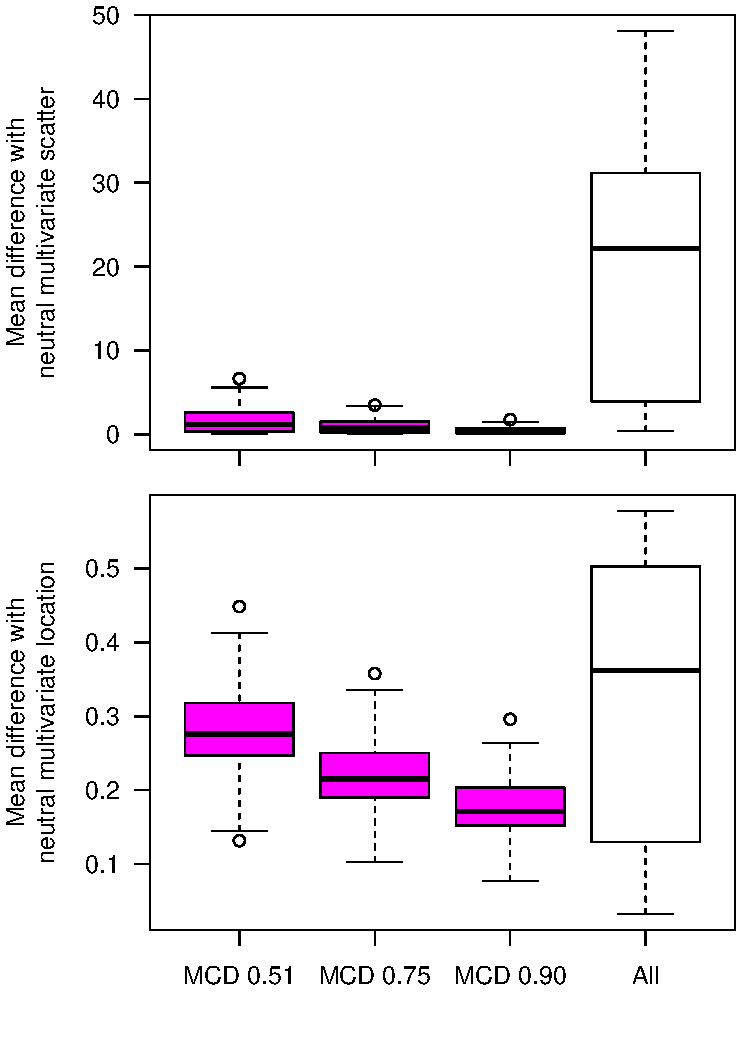
\includegraphics[height=6in]{../figures_man2/F1-LandsharcComparetoNeutlocationscatter.pdf}
\end{center}
\caption[]{ Mean difference between the estimate of location and scatter with the true neutral estimate. "All" refers to all the data (including selected loci), and MCD refers to the minimum covariance determinant estimate with the proportion of data used to create the subsets. Boxplots are summarized over all demographies and sampling designs.
} 
 \label{fig:???}
\end{figure}

\newpage
\begin{figure}[h]
\begin{center}
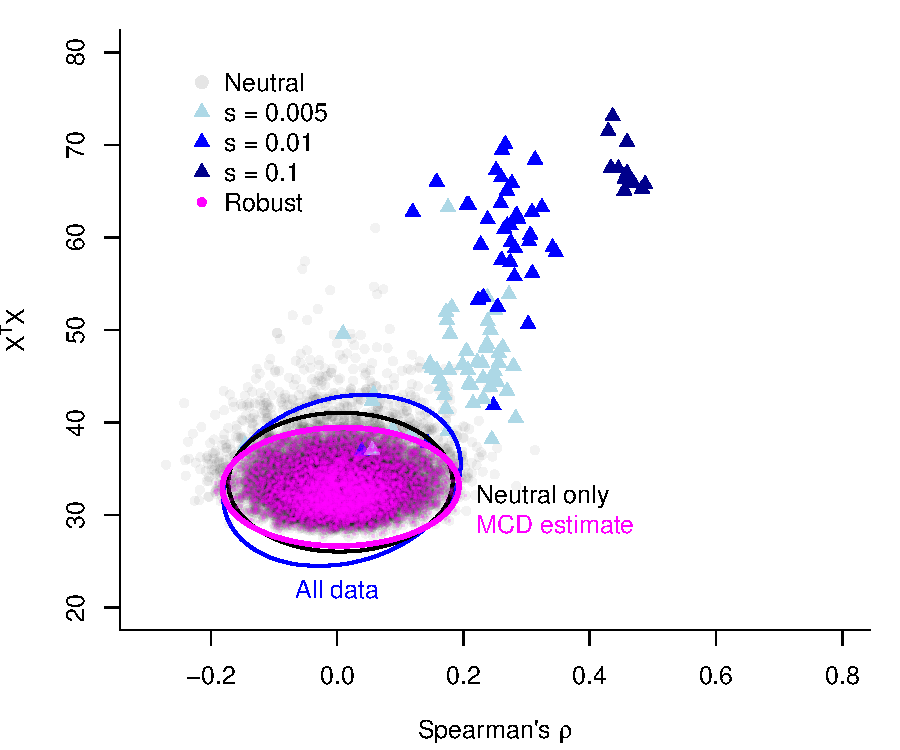
\includegraphics[width=3in]{../figures_man2/F2-VizCovariance.pdf}
\end{center}
\caption[]{Comparison of 95\% confidence intervals on the two dimensional ellipse given by the determinant on the covariance matrix between these two variables calculated from: (i) all the data, (ii) neutral loci only, and (iii) the MCD estimate.}
 \label{fig:???}
\end{figure}

\newpage
\begin{figure}[h]
\begin{center}
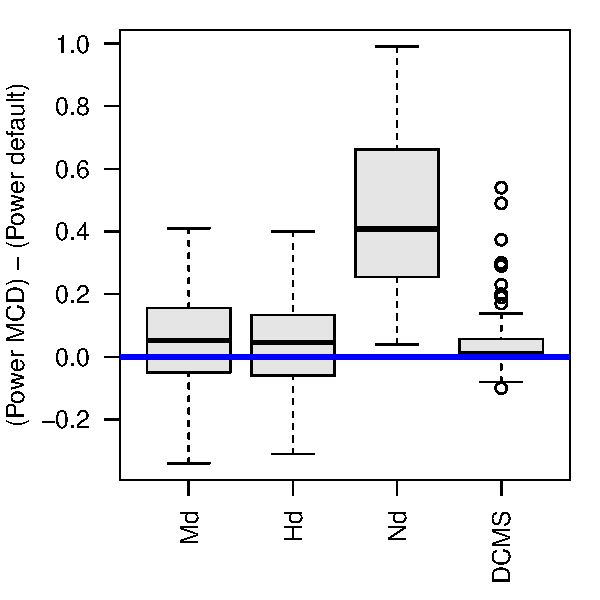
\includegraphics[width=3in]{../figures_man2/F3-LandsharcComparePowerMCDminusPowerDefault.pdf}
\end{center}
\caption[]{The difference in empirical power of the statistic to detect selection with and without the robust points identified by minimum covariance determinant (MCD) used in the calc ulation. Boxplots are summarized over all demographies.}
 \label{fig:???}
\end{figure}


\newpage
\begin{figure}[h]
\begin{center}
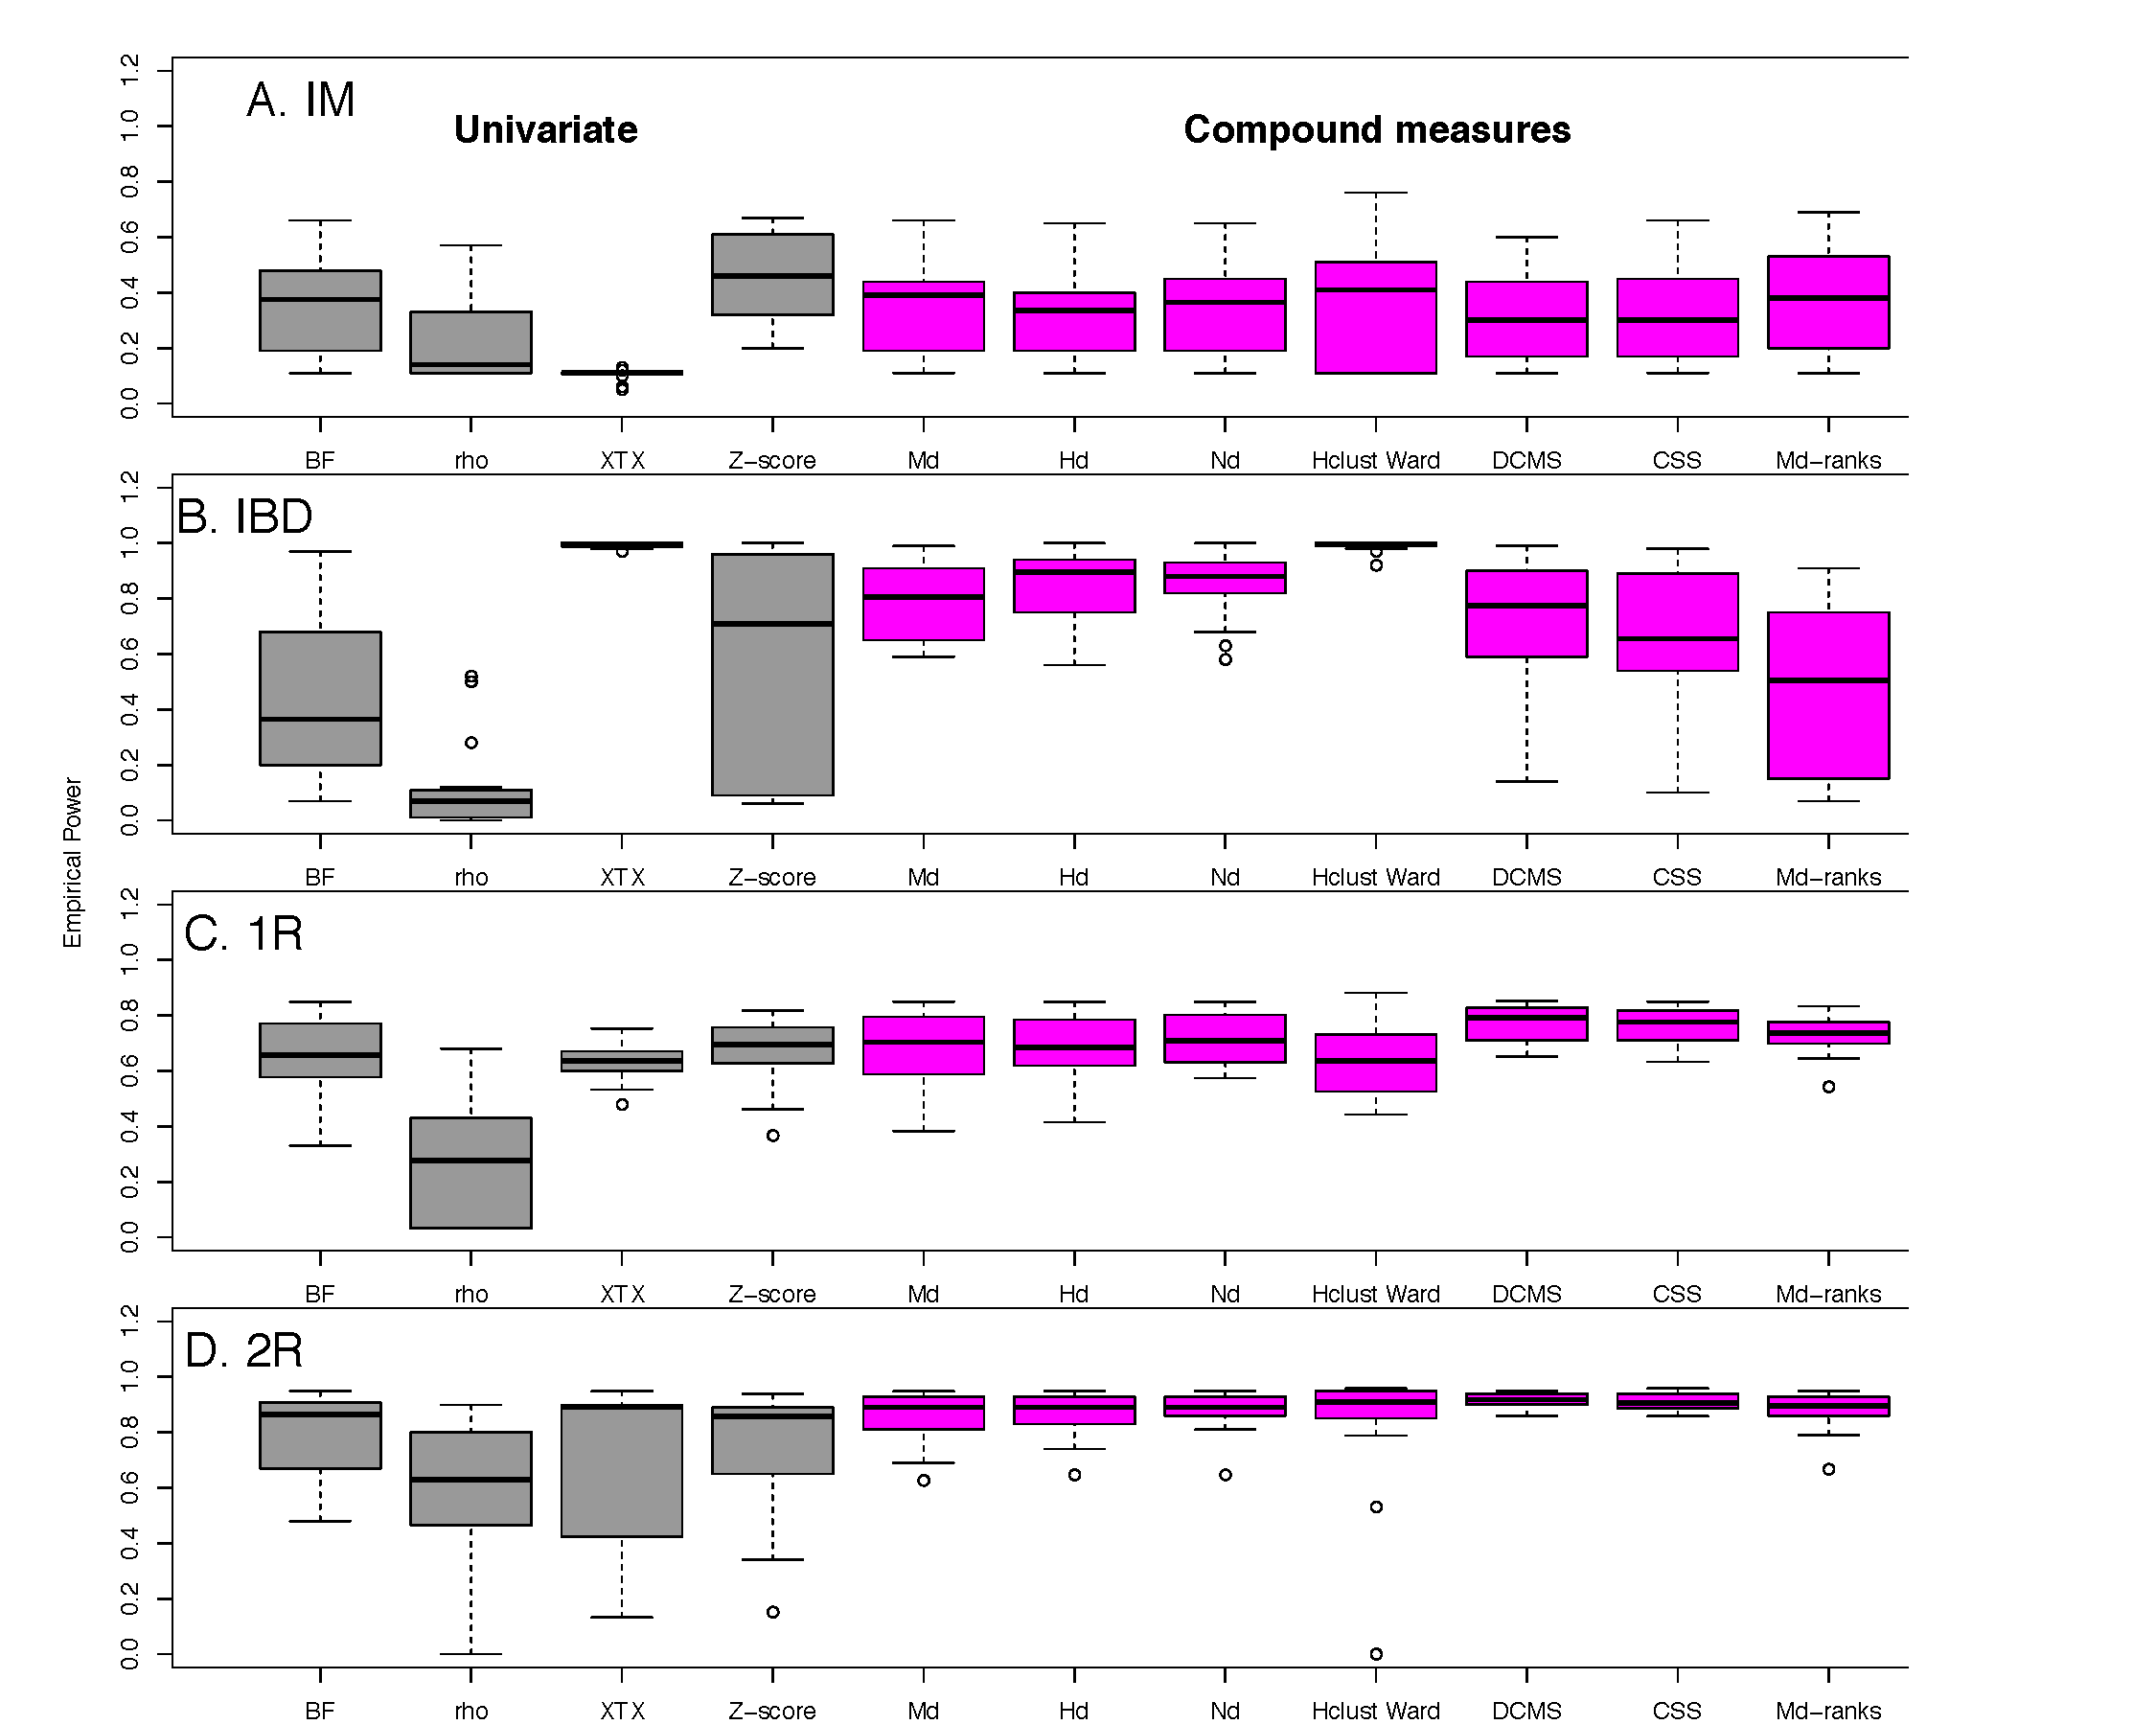
\includegraphics[width=6in]{../figures_man2/F4-LandsharcSummary2.pdf}
\end{center}
\caption[]{Comparison of empirical power of the univariate statistics and compound measures evaluated from the demography simulations. The univariate statistics include Bayes factor (BF) and Spearman's $\rho$ (rho) from a genetic-environment association, a measure of genetic diffentation (XTX), $Z$-score from the program LFMM.
The compound measures based on multivariate distances include: Mahalanobis distance (Md), harmonic mean distance (Hd), nearest neighbor distance (Nd), and hierarchical clustering (Hclust.Ward). The compound measures based on combining $P$-values include: decorrelated composite of multiple signals (DCMS), composite signal of selection (CSS), and Mahalanobis distance based on minus-log fractional $P$-values (Md-ranks).}
 \label{fig:???}
\end{figure}

\newpage
\begin{figure}[h]
\begin{center}
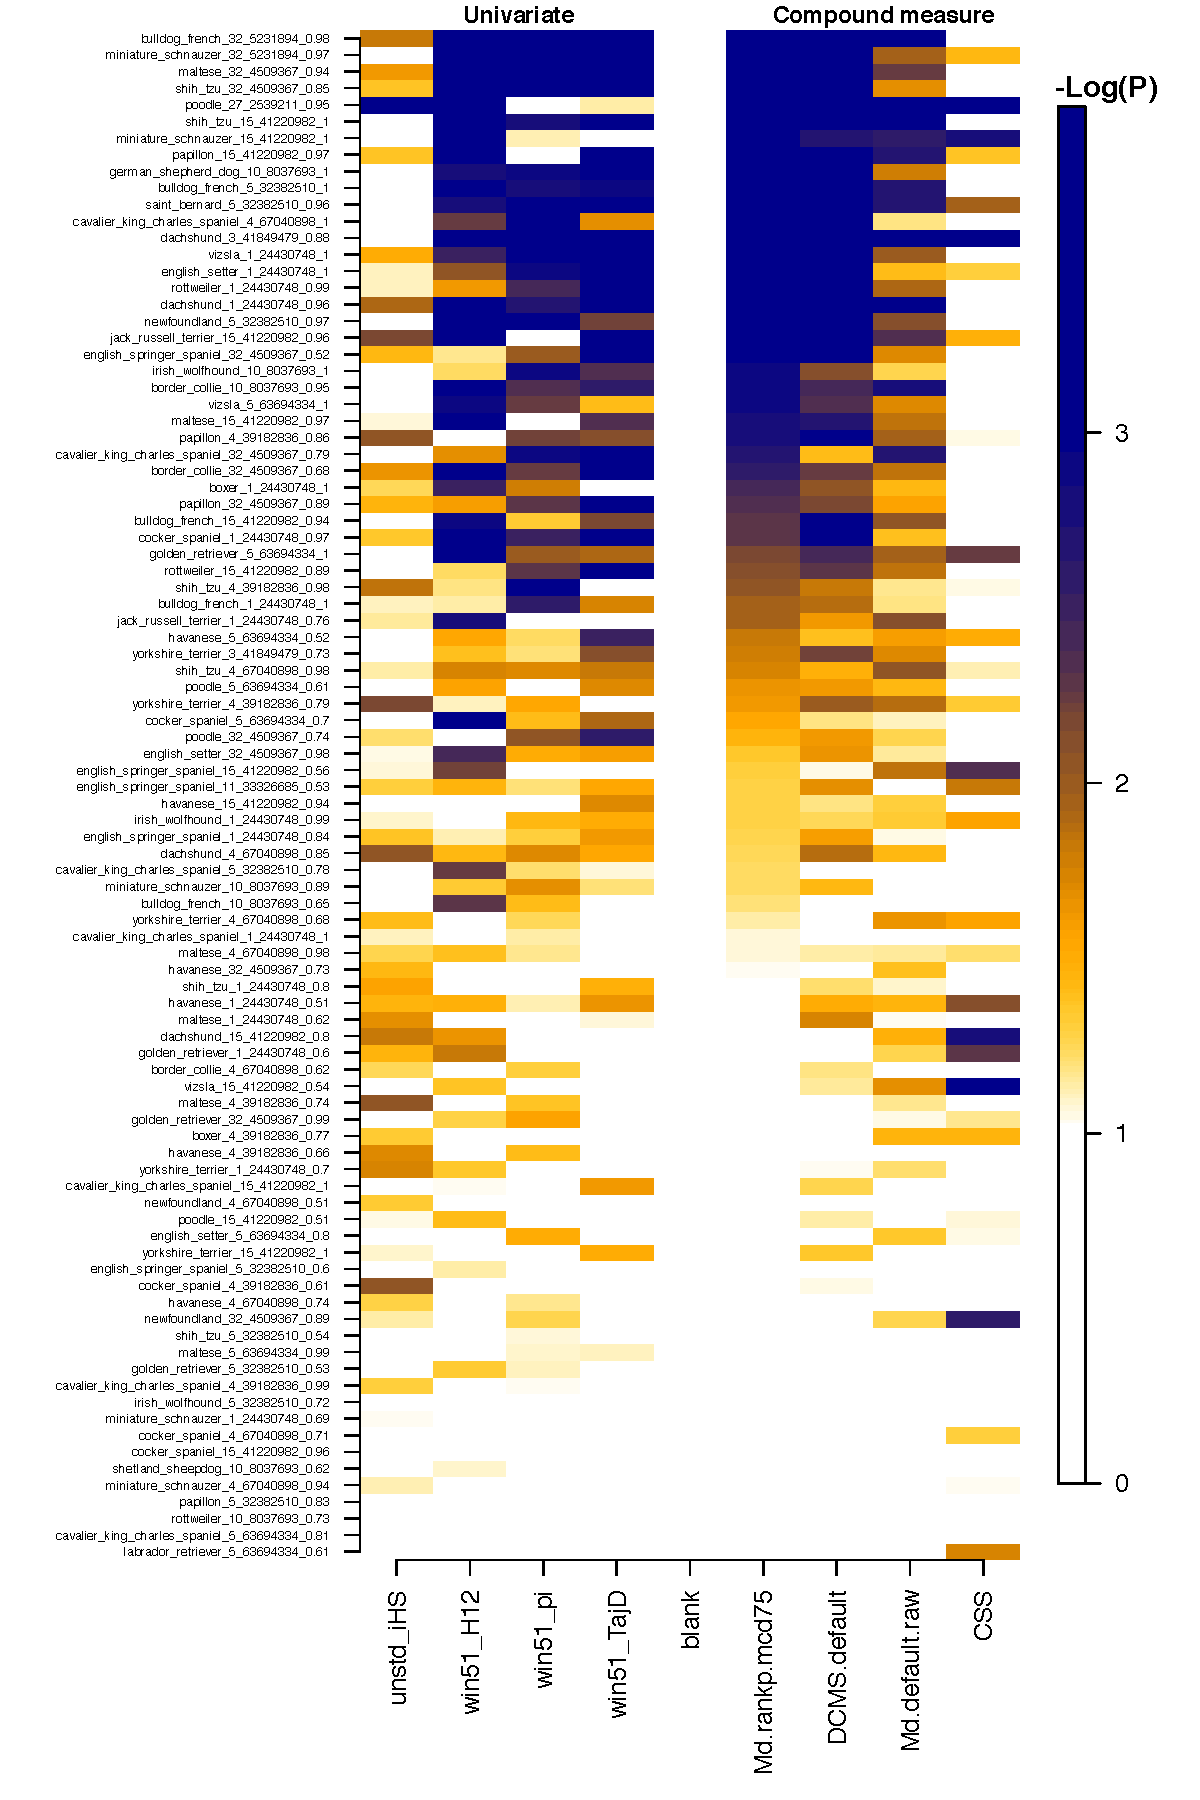
\includegraphics[height=6in]{../figures_man2/F5-Dog_heatmap_LogP_compare_stats.pdf}
\end{center}
\caption[]{Heatmap of statistical quantile based on a minus-log $P$-value calculated from ranks evaluated for each individual locus in the empirical dog dataset. The univariate statistics include iHS, H12, nucleotide diversity $\pi$, and Tajima's $D$. The compound measures include: the Mahalanobis distance based on minus-log fractional $P$-values (Md-rank-$P$), the decorrelated composite of multiple signals (DCMS), the Mahalanobis distance based on the raw statistics, and the composite signal of selection (CSS). The row labels indicate the dog breed, chromosome, base pair of the focal SNP, and the allele frequency of the focal SNP.

TO DO: EDIT X-AXIS LABELS}
 \label{fig:???}
\end{figure}


\newpage
\begin{figure}[h]
\begin{center}
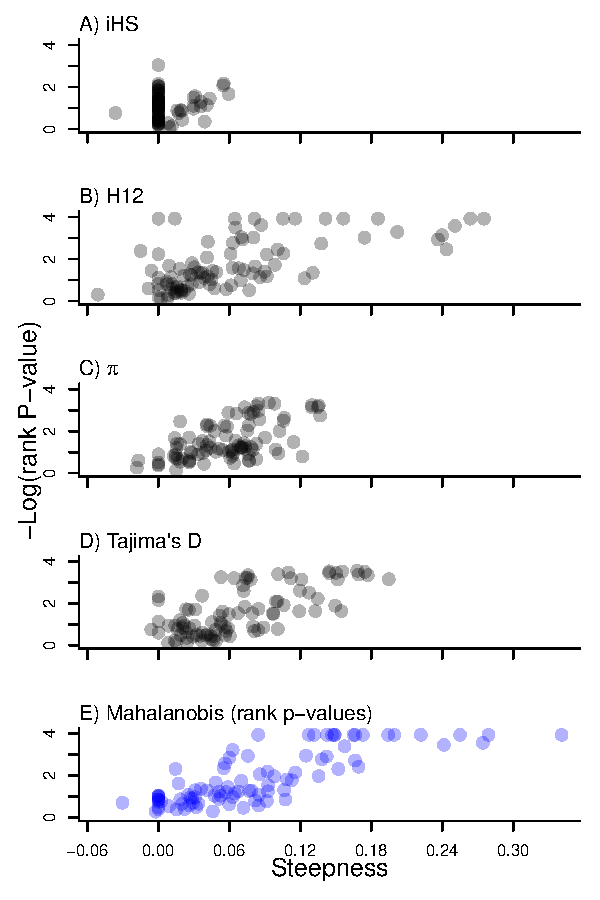
\includegraphics[height=6in]{../figures_man2/F6-Dog_ScatterCompareSteepnessAndEmp_UniMulti.pdf}
\end{center}
\caption[]{Statistical quantile based on a minus-log $P$-value calculated from ranks is plotted against steepness for each individual locus. Loci in the upper right hand of the graph have a steeper signal of selection and a more significant signal. The univariate statistics are plotted in A-D, compared to the Md-rank-$P$ plotted in E.}
 \label{fig:???}
\end{figure}

\end{document}